\chapter{Espectros eletrônicos e magnetismo dos complexos}\label{ch:b3:complex-spectra-magnetism}

O rubi é vermelho e a esmeralda é verde, mas ambos devem sua cor ao mesmo íon,
\ce{Cr^{3+}}, que substitui alguns íons alumínio em dois óxidos diferentes: o coríndon,
$\ce{Al2O3}$, no rubi, e o silicato de berílio e alumínio berilo, na esmeralda. Nos
dois, o crômio ocupa um octaedro de átomos de oxigênio; no berilo, o octaedro é um
pouco maior e o campo ligante um pouco mais fraco, e as bandas de absorção do íon se
deslocam cerca de mil números de onda para o vermelho. Isso basta para mudar a cor
transmitida de vermelho para verde. Este capítulo explica quantitativamente esses
espectros: como os termos de um íon livre se desdobram em um campo ligante, como os
\omterm{def:b3:complex-spectra-magnetism:tanabe-sugano}{diagramas de Tanabe--Sugano} transformam as posições de duas bandas no desdobramento
do campo ligante e na repulsão eletrônica, por que algumas bandas são intensas e
outras fracas, por que alguns complexos se distorcem e como o magnetismo conta os
elétrons desemparelhados.

\begin{recall}
O volume do 2.º ano tratou dos elementos de transição e de suas configurações $d^n$,
do desdobramento do campo cristalino $\Delta_{\mathrm o}$, dos complexos de spin alto e de spin
baixo, da energia de emparelhamento, da energia de estabilização do campo
cristalino, das transições $d$--$d$, da série espectroquímica, da teoria do campo
ligante e das substâncias paramagnéticas e diamagnéticas. O
\cref{ch:b3:many-electron-atoms} deduziu os \omterm{def:b3:many-electron-atoms:term}{símbolos de termo} e as regras de Hund,
o \cref{ch:b3:group-theory-applied} reduziu representações e \omterm{def:b3:group-theory-applied:direct-product}{produtos diretos}, o
\cref{ch:b3:electronic-spectroscopy} enunciou as regras de seleção de spin e de
Laporte e descreveu as transições de transferência de carga, e o
\cref{ch:b3:partition-functions} deu a \omterm{def:b3:partition-functions:boltzmann}{distribuição de Boltzmann}.
\end{recall}

\begin{omfigure}
\begin{minipage}[b]{0.3\linewidth}\centering
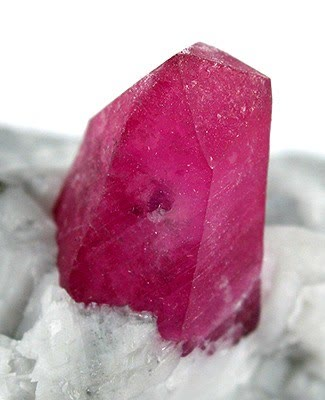
\includegraphics[height=4.2cm]{images/book4/ruby-crystal.jpg}\par
{\small rubi}
\end{minipage}\hspace{1.5em}
\begin{minipage}[b]{0.3\linewidth}\centering
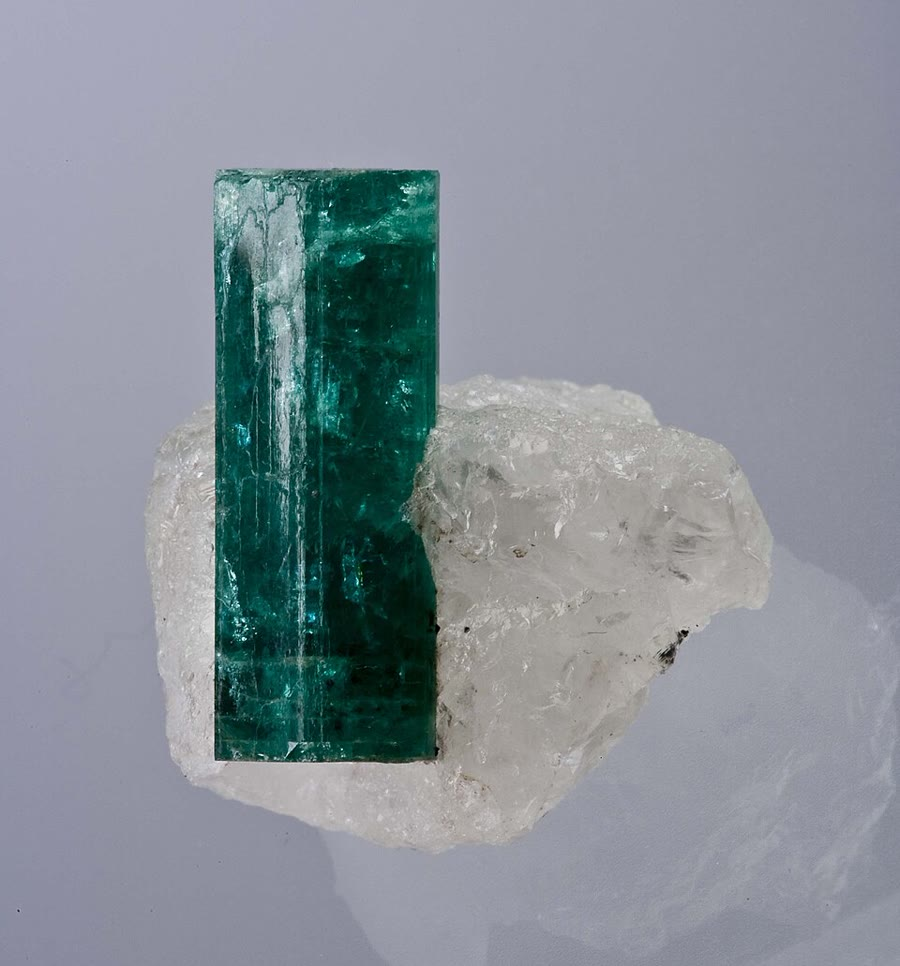
\includegraphics[height=4.2cm]{images/book4/emerald-crystal.jpg}\par
{\small esmeralda}
\end{minipage}

{\small Um cristal de rubi em mármore e um cristal de esmeralda sobre quartzo. Nos
dois, a cor vem de alguns por cento de \ce{Cr^{3+}} em um sítio octaédrico.}
\end{omfigure}

\section{Dos termos do íon livre aos termos do campo ligante}

Em um íon livre, a repulsão eletrônica desdobra uma configuração $d^n$ em termos
($^4$F, $^4$P, $^2$G\dots\ para $d^3$, \cref{ch:b3:many-electron-atoms}). Em um complexo,
cada termo é ainda desdobrado pelos ligantes, e os níveis são rotulados pelas
\omterm{def:b3:point-groups:irrep}{representações irredutíveis} do \omterm{def:b3:point-groups:point-group}{grupo pontual} do complexo.

\begin{definition}[Termo do campo ligante]\label{def:b3:complex-spectra-magnetism:ligand-field-term}
Um \emph{termo do campo ligante}\index{termo do campo ligante} de um complexo é um conjunto de
estados polieletrônicos degenerados rotulados por sua \omterm{def:b3:many-electron-atoms:term}{multiplicidade de spin} e pela
\omterm{def:b3:point-groups:irrep}{representação irredutível} do \omterm{def:b3:point-groups:point-group}{grupo pontual} à qual pertence sua parte orbital, como
$^4$A$_{2g}$ ou $^4$T$_{1g}$ em um complexo octaédrico.
\end{definition}

\begin{proposition}[Caracteres do grupo das rotações]\label{prop:b3:complex-spectra-magnetism:rotation-characters}
Os $2L+1$ estados de um termo de momento angular orbital $L$ formam uma representação
das rotações cujo \omterm{def:b3:point-groups:representation}{caráter} para uma rotação de $\alpha$ é
\[
  \chi_L(\alpha) = \frac{\sin\bigl((L + \tfrac12)\alpha\bigr)}{\sin(\alpha/2)}, \qquad \chi_L(0) = 2L + 1 .
\]
\end{proposition}

\admitted

\begin{theorem}[Desdobramento dos termos do íon livre em um campo octaédrico]\label{thm:b3:complex-spectra-magnetism:term-splitting}
Em um campo octaédrico, os termos de um íon $d^n$ se desdobram em
\begin{center}
\begin{tabular}{ll}
\hline
termo do íon livre & termos octaédricos (mesma \omterm{def:b3:many-electron-atoms:term}{multiplicidade de spin}) \\ \hline
S & A$_{1g}$ \\
P & T$_{1g}$ \\
D & E$_g$ + T$_{2g}$ \\
F & A$_{2g}$ + T$_{1g}$ + T$_{2g}$ \\
G & A$_{1g}$ + E$_g$ + T$_{1g}$ + T$_{2g}$ \\ \hline
\end{tabular}
\end{center}
\end{theorem}

\begin{proof}
O grupo octaédrico é o grupo das rotações $O$ vezes a inversão; as funções $d$ são
pares, de modo que todo termo de uma configuração $d^n$ é par ($g$), e basta reduzir
em $O$, cujas classes são $E$, $8C_3$, $3C_2$ ($=C_4^2$), $6C_4$ e $6C_2'$. Com a
proposição, para $L = 3$: $\chi = 7$, $\sin(420^\circ)/\sin60^\circ = 1$, $\sin(630^\circ)/\sin90^\circ = -1$, $\sin(315^\circ)/\sin45^\circ = -1$
e $-1$. A \omterm{def:b3:point-groups:irrep}{tabela de caracteres} de $O$ (linhas $A_1$: 1, 1, 1, 1, 1; $A_2$: 1, 1, 1, $-1$, $-1$; $E$: 2,
$-1$, 2, 0, 0; $T_1$: 3, 0, $-1$, 1, $-1$; $T_2$: 3, 0, $-1$, $-1$, 1) e a \omterm{thm:b3:group-theory-applied:reduction}{fórmula de redução} do
\cref{ch:b3:group-theory-applied} dão $n(A_2) = (7 + 8 - 3 + 6 + 6)/24 = 1$, $n(T_1) = (21 + 3 - 6 +
6)/24 = 1$, $n(T_2) = (21 + 3 + 6 - 6)/24 = 1$, e zero para $A_1$ e $E$. As outras linhas são
obtidas da mesma maneira ($L = 0$: $(1, 1, 1, 1, 1)$; $L = 1$: $(3, 0, -1, 1, -1)$; $L = 2$: $(5, -1, 1,
-1, 1)$; $L = 4$: $(9, 0, 1, 1, 1)$).
\end{proof}

\begin{method}[Desdobrar um termo do íon livre]\label{met:b3:complex-spectra-magnetism:split-term}
\begin{enumerate}
  \item Encontre o termo fundamental do íon livre (regras de Hund) e os termos
        excitados de mesma multiplicidade.
  \item Leia na tabela suas componentes octaédricas; a \omterm{def:b3:many-electron-atoms:term}{multiplicidade de spin} não
        muda.
  \item Ordene-as: para o termo F fundamental de $d^2$, $d^7$ (spin alto), a mais baixa é T$_{1g}$;
        para $d^3$, $d^8$, é A$_{2g}$ (proposição seguinte).
\end{enumerate}
\end{method}

\begin{proposition}[Buracos e inversão tetraédrica]\label{prop:b3:complex-spectra-magnetism:hole}
Os termos de $d^{10-n}$ em um campo octaédrico são os de $d^n$ em ordem de energia
invertida; os termos de $d^n$ em um campo tetraédrico são os de $d^{10-n}$ em um campo
octaédrico (sem os índices $g$).
\end{proposition}

\begin{proof}
Uma configuração $d^{10-n}$ equivale a $n$ buracos positivos em uma camada completa: os
buracos sentem o potencial do campo ligante com o sinal oposto, de modo que todo
desdobramento monoeletrônico, e logo todo desdobramento de termo, é invertido (a
repulsão eletrônica entre buracos é a mesma que entre elétrons). Um campo
tetraédrico tem o sinal oposto ao de um campo octaédrico (os orbitais $e$ ficam
mais baixos) e não tem centro de simetria: $d^n$ em $T_d$ se comporta como $d^n$ com um
campo invertido, isto é, como $d^{10-n}$ em $O_h$.
\end{proof}

\begin{definition}[Diagrama de correlação]\label{def:b3:complex-spectra-magnetism:correlation}
Um \emph{diagrama de correlação}\index{diagrama de correlacao@diagrama de correlação} liga os estados de um
sistema em duas situações-limite, aqui os termos do íon livre desdobrados por um
campo fraco e as configurações $t_{2g}^ae_g^b$ de um campo forte, unindo estados de mesma
simetria sem deixar que dois deles se cruzem.
\end{definition}

\begin{omfigure}
\begin{tikzpicture}[font=\small]
  % free ion
  \pic (F) at (0,0) {omlevel={}{1.1}};
  \pic (P) at (0,3.0) {omlevel={}{1.1}};
  \node[anchor=east] at (F-l) {$^3$F};
  \node[anchor=east] at (P-l) {$^3$P};
  % weak field
  \pic (a) at (2.6,-0.8) {omlevel={}{1.0}};
  \pic (b) at (2.6,0.3) {omlevel={}{1.0}};
  \pic (c) at (2.6,1.4) {omlevel={}{1.0}};
  \pic (d) at (2.6,3.1) {omlevel={}{1.0}};
  \foreach \n/\t in {a/T$_{1g}$, b/T$_{2g}$, c/A$_{2g}$, d/T$_{1g}$(P)}{\node[omsymlabel, anchor=south] at (\n-c) {$^3$\t};}
  \draw[omcorr] (F-r) -- (a-l) (F-r) -- (b-l) (F-r) -- (c-l) (P-r) -- (d-l);
  % strong field configurations
  \pic (A) at (7.4,-1.6) {omlevel={}{1.0}};
  \pic (B) at (7.4,1.4) {omlevel={}{1.0}};
  \pic (C) at (7.4,1.9) {omlevel={}{1.0}};
  \pic (D) at (7.4,4.6) {omlevel={}{1.0}};
  \node[anchor=west] at (A-r) {$^3$T$_{1g}$ \quad $t_{2g}^2$};
  \node[anchor=west] at (B-r) {$^3$T$_{2g}$};
  \node[anchor=west] at (C-r) {$^3$T$_{1g}$ \quad $t_{2g}e_g$};
  \node[anchor=west] at (D-r) {$^3$A$_{2g}$ \quad $e_g^2$};
  \draw[omcorr] (a-r) -- (A-l) (b-r) -- (B-l) (c-r) -- (D-l) (d-r) -- (C-l);
  \node[anchor=north] at (0,-2.0) {íon livre};
  \node[anchor=north] at (2.6,-2.0) {campo fraco};
  \node[anchor=north] at (7.4,-2.0) {campo forte};
  \draw[->, black!50] (3.7,-2.3) -- (6.2,-2.3) node[midway, below, font=\scriptsize] {$\Delta_{\mathrm o}$ crescente};
\end{tikzpicture}

{\small \omterm{def:b3:complex-spectra-magnetism:correlation}{Diagrama de correlação} dos \omterm{def:b3:many-electron-atoms:singlet-triplet}{estados tripleto} de um íon $d^2$ em um campo
octaédrico. Cada termo de campo fraco vai para a configuração de campo forte de mesma
simetria, e os dois estados $^3$T$_{1g}$ não se cruzam: o mais baixo vai para $t_{2g}^2$, o mais
alto para $t_{2g}e_g$.}
\end{omfigure}

\section{Diagramas de Tanabe--Sugano}

\begin{definition}[Parâmetros de Racah]\label{def:b3:complex-spectra-magnetism:racah}
Os \emph{parâmetros de Racah}\index{parametros de Racah@parâmetros de Racah} $A$, $B$ e $C$ são combinações das
integrais de Slater da camada $d$ que exprimem todas as energias de repulsão
eletrônica de uma configuração $d^n$; as diferenças de energia entre termos da mesma
configuração dependem apenas de $B$ e $C$, e as entre termos da mesma multiplicidade
máxima, apenas de $B$ (para $d^2$, $d^3$, $d^7$, $d^8$: $E(\mathrm P) - E(\mathrm F) = 15B$).
\end{definition}

\begin{example}[Parâmetros de Racah do íon livre]\label{ex:b3:complex-spectra-magnetism:free-B}
% ledger: lev:Cr3.4F5_2, lev:Cr3.4F7_2, lev:Cr3.4F9_2, lev:Cr3.4P1_2, lev:Cr3.4P3_2, lev:Cr3.4P5_2, lev:Ni2.3F3, lev:Ni2.3F2, lev:Ni2.3P2, lev:Ni2.3P1, lev:Ni2.3P0, lev:V2.4F5_2, lev:V2.4F7_2, lev:V2.4F9_2, lev:V2.4P1_2, lev:V2.4P3_2, lev:V2.4P5_2
Os níveis do íon \ce{Cr^{3+}} livre põem o baricentro (pesos $2J + 1$) de $^4$F a
\qty{547}{cm^{-1}} e o de $^4$P a \qty{14305}{cm^{-1}} acima do nível fundamental: $15B = \qty{13758}{cm^{-1}}$,
$B = \qty{917}{cm^{-1}}$. O mesmo cálculo dá $B = 755$ para \ce{V^{2+}} e \qty{1056}{cm^{-1}} para
\ce{Ni^{2+}}.
\end{example}

\begin{definition}[Diagrama de Tanabe--Sugano]\label{def:b3:complex-spectra-magnetism:tanabe-sugano}
Um \emph{diagrama de Tanabe--Sugano}\index{diagrama de Tanabe--Sugano} representa as energias de
todos os \omterm{def:b3:complex-spectra-magnetism:ligand-field-term}{termos do campo ligante} de um íon $d^n$, em unidades de $B$ e medidas a partir
do termo fundamental, em função de $\Delta_{\mathrm o}/B$, para uma razão $C/B$ fixa.
\end{definition}

\begin{proposition}[As três bandas de um íon $d^3$]\label{prop:b3:complex-spectra-magnetism:d3-bands}
Para um íon $d^3$ em um campo octaédrico, as transições permitidas por spin a partir de $^4$A$_{2g}$ ficam em
\[
  \nu_1 = \Delta_{\mathrm o}\ (^4\mathrm T_{2g}), \qquad
  \nu_{2,3} = 7.5B + 1.5\Delta_{\mathrm o} \mp \tfrac12\sqrt{225B^2 - 18B\Delta_{\mathrm o} + \Delta_{\mathrm o}^2}\ (^4\mathrm T_{1g}(\mathrm F), {}^4\mathrm T_{1g}(\mathrm P)).
\]
\end{proposition}

\begin{proof}[Demonstração parcial]
Na base de campo forte, $^4$A$_{2g}$ e $^4$T$_{2g}$ aparecem uma vez cada, a partir de $t_{2g}^3$ e de $t_{2g}^2e_g$, e
sua diferença não contém repulsão eletrônica: $\nu_1 = \Delta_{\mathrm o}$ exatamente. $^4$T$_{1g}$ aparece
duas vezes, a partir de $t_{2g}^2e_g$ e de $t_{2g}e_g^2$; em relação a $^4$A$_{2g}$, a matriz $2\times2$ é
$\begin{pmatrix}\Delta_{\mathrm o} + 12B & 6B\\ 6B & 2\Delta_{\mathrm o} + 3B\end{pmatrix}$ (os elementos de repulsão eletrônica são admitidos).
Seus \omterm{def:b3:quantum-model-systems:operator}{autovalores} são as raízes de $E^2 - (15B + 3\Delta_{\mathrm o})E + 2\Delta_{\mathrm o}^2 + 27B\Delta_{\mathrm o} = 0$, que são os
$\nu_2$ e $\nu_3$ enunciados. Em $\Delta_{\mathrm o} = 0$, eles valem 0 e $15B$ (os termos $^4$F e $^4$P); a
diagonalização completa da figura os reproduz.
\end{proof}

\begin{omfigure}
\begin{tikzpicture}
\begin{axis}[name=ta, omts, width=0.46\linewidth, height=7.0cm, xmin=1, xmax=40, ymin=0, ymax=70,
  xlabel={$\Delta_{\mathrm o}/B$}, ylabel={$E/B$}, title={\small $d^3$, $C/B = 4.5$},
  unbounded coords=jump, clip=true, clip mode=individual]
\foreach \c in {f0,f1,f2,f3,f4,f5,f6,f7,f8,f9,f10,f11,f12,f13,f14,f15}{
  \addplot[omtsforbidden, restrict x to domain=1:40] table[x=x, y=\c] {figdata/out/bachelor-3-tanabe-sugano-d3.dat};}
\foreach \c in {a0,a1,a2,a3}{
  \addplot[omDef, thick, restrict x to domain=1:40] table[x=x, y=\c] {figdata/out/bachelor-3-tanabe-sugano-d3.dat};}
\draw[omThm, dashed] (axis cs:29.0,0) -- (axis cs:29.0,70);
\draw[black!70, dashed] (axis cs:27.1,0) -- (axis cs:27.1,70);
\node[font=\scriptsize, omThm, anchor=north west, rotate=90] at (axis cs:29.6,1.5) {rubi};
\node[font=\scriptsize, anchor=south west, rotate=90] at (axis cs:26.6,1.5) {esmeralda};
% labels outside the frame, at the height where each curve leaves it
\node[font=\scriptsize, omDef, anchor=west, inner sep=1pt] at (axis cs:40,40) {$^4$T$_{2g}$};
\node[font=\scriptsize, omDef, anchor=west, inner sep=1pt] at (axis cs:40,50.9) {$^4$T$_{1g}$};
\node[font=\scriptsize, omDef, anchor=south, inner sep=1pt] at (axis cs:32.8,70) {$^4$T$_{1g}$(P)};
\node[font=\scriptsize, black!60, anchor=west, inner sep=1pt] at (axis cs:40,21.2) {$^2$E$_g$};
\end{axis}
\begin{axis}[at={(ta.east)}, anchor=west, xshift=2.2cm, omts, width=0.46\linewidth, height=7.0cm,
  xmin=1, xmax=40, ymin=0, ymax=70, xlabel={$\Delta_{\mathrm o}/B$}, ylabel={$E/B$},
  title={\small $d^8$, $C/B = 4.71$}, unbounded coords=jump, clip=true, clip mode=individual]
\foreach \c in {f0,f1,f2,f3,f4,f5,f6}{
  \addplot[omtsforbidden, restrict x to domain=1:40] table[x=x, y=\c] {figdata/out/bachelor-3-tanabe-sugano-d8.dat};}
\foreach \c in {a0,a1,a2,a3}{
  \addplot[omDef, thick, restrict x to domain=1:40] table[x=x, y=\c] {figdata/out/bachelor-3-tanabe-sugano-d8.dat};}
\node[font=\scriptsize, omDef, anchor=west, inner sep=1pt] at (axis cs:40,40) {$^3$T$_{2g}$};
\node[font=\scriptsize, omDef, anchor=west, inner sep=1pt] at (axis cs:40,50.9) {$^3$T$_{1g}$};
\node[font=\scriptsize, omDef, anchor=south, inner sep=1pt] at (axis cs:32.8,70) {$^3$T$_{1g}$(P)};
\end{axis}
\end{tikzpicture}

{\small \omterm{def:b3:complex-spectra-magnetism:tanabe-sugano}{Diagramas de Tanabe--Sugano} de íons $d^3$ e $d^8$ calculados pela diagonalização
do hamiltoniano de campo ligante e de repulsão eletrônica sobre todos os estados da
configuração. Em azul e grosso: os estados da multiplicidade do estado fundamental
(transições permitidas por spin); em cinza e fino: os demais. O termo fundamental é o
eixo horizontal ($^4$A$_{2g}$ para $d^3$, $^3$A$_{2g}$ para $d^8$). Tracejados: o rubi e a esmeralda, situados no $\Delta_{\mathrm o}/B$ de suas duas bandas.
O nível $^2$E$_g$ de $d^3$ é quase plano: sua energia quase não depende do campo.}
\end{omfigure}

\begin{method}[Ler um diagrama de Tanabe--Sugano]\label{met:b3:complex-spectra-magnetism:read-ts}
\begin{enumerate}
  \item Identifique o termo fundamental e as transições permitidas por spin (mesma
        multiplicidade).
  \item Calcule a razão entre as energias de duas bandas, $\nu_2/\nu_1$; encontre o valor de
        $\Delta_{\mathrm o}/B$ no qual o diagrama dá essa razão.
  \item Leia ali $E/B$ para $\nu_1$: $B = \nu_1/(E/B)$, e depois $\Delta_{\mathrm o}$. Para $d^3$ e $d^8$, $\Delta_{\mathrm o} = \nu_1$
        diretamente, e a fórmula fechada dá $B$ a partir de $\nu_2$.
  \item Compare $B$ com o valor do íon livre (\omterm{def:b3:complex-spectra-magnetism:nephelauxetic}{razão nefelauxética}) e verifique que a
        terceira banda cai onde o diagrama prevê.
\end{enumerate}
\end{method}

\begin{definition}[Efeito nefelauxético]\label{def:b3:complex-spectra-magnetism:nephelauxetic}
O \emph{efeito nefelauxético}\index{efeito nefelauxetico@efeito nefelauxético} (``que expande a nuvem'') é a
diminuição do parâmetro de Racah $B$ de um íon metálico em um complexo em relação ao
íon livre, causada pela deslocalização dos elétrons $d$ sobre os ligantes; a
\emph{razão nefelauxética}\index{razao nefelauxetica@razão nefelauxética} é $\beta =
B_{\text{complexo}}/B_{\text{íon livre}}$.
\end{definition}

Os ligantes que se ligam de modo mais covalente reduzem mais $B$: $\beta$ fica perto de
0.9 para o fluoreto, 0.8 para a água, 0.6 a 0.7 para o óxido e os haletos mais
pesados, e ainda menos para o sulfeto. As transições proibidas por spin, entre termos
de multiplicidades diferentes, aparecem como raias fracas, muitas vezes finas.

\section{Intensidades e transferência de carga}

\begin{definition}[Acoplamento vibrônico]\label{def:b3:complex-spectra-magnetism:vibronic-coupling}
O \emph{acoplamento vibrônico}\index{acoplamento vibronico@acoplamento vibrônico} é a mistura dos movimentos
eletrônico e vibracional: uma vibração assimétrica que remove o centro de simetria
de um complexo mistura um pouco de caráter ímpar ($u$) a seus estados $d$, o que torna
fracamente permitidas as transições $d$--$d$ proibidas por Laporte.
\end{definition}

\begin{proposition}[Intensidades das bandas de absorção]\label{prop:b3:complex-spectra-magnetism:intensity-order}
Os coeficientes de absorção molar das bandas dos complexos crescem na ordem:
$d$--$d$ proibida por spin $\ll$ $d$--$d$ permitida por spin em um complexo centrossimétrico $<$ $d$--$d$
em um complexo tetraédrico $<$ transferência de carga.
\end{proposition}

\begin{proof}[Argumento]
Pelo \cref{ch:b3:electronic-spectroscopy}, uma transição é permitida quando o spin é
conservado e a paridade muda. Uma transição $d$--$d$ nunca muda a paridade: em um
complexo octaédrico, ela só toma intensidade emprestada por \omterm{def:b3:complex-spectra-magnetism:vibronic-coupling}{acoplamento vibrônico}; em
um tetraedro, que não tem centro, os orbitais $d$ e $p$ se misturam permanentemente.
Uma transição proibida por spin toma emprestada ainda uma pequena fração por meio do
\omterm{def:b3:many-electron-atoms:spin-orbit}{acoplamento spin--órbita}. Uma \omterm{def:b3:electronic-spectroscopy:charge-transfer}{transição de transferência de carga} leva um elétron
entre orbitais de paridades diferentes no metal e no ligante, e é plenamente permitida.
\end{proof}

\begin{definition}[Transferência de carga]\label{def:b3:complex-spectra-magnetism:ct}
Em uma \emph{transferência de carga ligante--metal}\index{transferencia de carga ligante--metal@transferência de carga ligante--metal}
(LMCT), um elétron passa de um orbital centrado no ligante para um orbital centrado no
metal; em uma \emph{transferência de carga metal--ligante}\index{transferencia de carga metal--ligante@transferência de carga metal--ligante}
(MLCT), do metal para um orbital $\pi^*$ do ligante.
\end{definition}

O permanganato e o cromato, íons $d^0$ sem nenhuma transição $d$--$d$, devem suas cores
intensas a uma LMCT do óxido para um orbital $d$ vazio do metal, fácil para um metal em
estado de oxidação alto. O $\ce{[Ru(bpy)3]^{2+}}$ (bpy: 2,2$'$-bipiridina) deve sua cor laranja a uma MLCT
do rutênio(II) para os orbitais $\pi^*$ dos ligantes, o estado excitado usado na \omterm{def:b3:photochemistry:photoredox}{catálise
fotorredox} (\cref{ch:b3:photochemistry}). No rubi, as duas bandas largas perto de 560 e
\qty{410}{nm} são as bandas $d$--$d$ permitidas por spin da
\cref{prop:b3:complex-spectra-magnetism:d3-bands}; a luz que passa é vermelha, com um
pouco de azul. Excitado nessas bandas, o íon relaxa para o nível $^2$E$_g$ e emite a partir
dele a raia R, vermelho-escura, perto de \qty{695}{nm}, a raia do primeiro laser.

\section{O efeito Jahn--Teller}

\begin{theorem}[Teorema de Jahn--Teller]\label{thm:b3:complex-spectra-magnetism:jahn-teller}
Uma molécula não linear em um estado eletrônico orbitalmente degenerado é instável em
relação a uma distorção que abaixa sua simetria e remove a \omterm{def:b3:quantum-model-systems:degenerate}{degenerescência}. Este é o
\emph{teorema de Jahn--Teller}\index{teorema de Jahn--Teller}.
\end{theorem}

\admitted

Suas consequências para os complexos octaédricos decorrem da ocupação dos orbitais
$e_g$, que apontam para os ligantes. Em um íon $d^9$ (\ce{Cu^{2+}}), a configuração
$t_{2g}^6e_g^3$ tem o buraco em $d_{z^2}$ ou em $d_{x^2-y^2}$: um estado E$_g$. Alongar as duas
ligações axiais abaixa $d_{z^2}$ e eleva $d_{x^2-y^2}$; pôr dois elétrons no orbital abaixado
e um no orbital elevado dá uma estabilização líquida. Os complexos de cobre(II) são de
fato octaedros alongados, com quatro ligações curtas e duas longas. O mesmo vale para
$d^4$ de spin alto (\ce{Mn^{3+}}, \ce{Cr^{2+}}) e $d^7$ de spin baixo; para conjuntos $t_{2g}$ preenchidos de
modo desigual ($d^1$, $d^2$, $d^5$ de spin baixo\dots), os orbitais apontam entre os
ligantes e a distorção é pequena. Os estados excitados degenerados dos complexos
também se distorcem: as bandas largas, muitas vezes com dois máximos, de
\ce{[Ti(H2O)6]^{3+}} e dos complexos de cobre(II) são sua assinatura espectroscópica.

\begin{omfigure}
\begin{tikzpicture}[font=\small]
  \pic[transform shape] (t) at (0,0) {omlevel={}{1.6}};
  \pic[transform shape] (e) at (0,2.2) {omlevel={}{1.1}};
  \node[anchor=east] at (t-l) {$t_{2g}$};
  \node[anchor=east] at (e-l) {$e_g$};
  \pic[transform shape] (xy) at (4.2,0.45) {omlevel={ud}{0.8}};
  \pic[transform shape] (xz) at (4.2,-0.25) {omlevel={ud}{1.4}};
  \pic[transform shape] (x2) at (4.2,3.0) {omlevel={u}{0.8}};
  \pic[transform shape] (z2) at (4.2,1.5) {omlevel={ud}{0.8}};
  \draw[omcorr] (t-r) -- (xy-l) (t-r) -- (xz-l) (e-r) -- (x2-l) (e-r) -- (z2-l);
  \node[anchor=west] at (xy-r) {$b_{2g}$ ($d_{xy}$)};
  \node[anchor=west] at (xz-r) {$e_g$ ($d_{xz}$, $d_{yz}$)};
  \node[anchor=west] at (x2-r) {$b_{1g}$ ($d_{x^2-y^2}$)};
  \node[anchor=west] at (z2-r) {$a_{1g}$ ($d_{z^2}$)};
  \node[anchor=north] at (0,-0.9) {$O_h$};
  \node[anchor=north] at (4.2,-0.9) {$D_{4h}$, alongado};
  \begin{scope}[xshift=9.0cm, yshift=1.2cm, scale=0.8]
    \pic[transform shape] {omoctahedron};
    \draw[->, thick, omThm] (0,1.25) -- (0,1.85);
    \draw[->, thick, omThm] (0,-1.25) -- (0,-1.85);
  \end{scope}
\end{tikzpicture}

{\small Distorção de Jahn--Teller de um complexo octaédrico $d^9$: alongar as ligações axiais (à direita) desdobra $e_g$ em $a_{1g}$
($d_{z^2}$, abaixado) e $b_{1g}$ ($d_{x^2-y^2}$, elevado), e $t_{2g}$ em $e_g$ e $b_{2g}$. Com nove
elétrons, o único buraco fica em $b_{1g}$: a distorção é uma estabilização líquida.}
\end{omfigure}

\section{Magnetismo}

\begin{definition}[Suscetibilidade magnética]\label{def:b3:complex-spectra-magnetism:susceptibility}
A \emph{suscetibilidade magnética}\index{suscetibilidade magnetica@suscetibilidade magnética} $\chi$ de um material
é a razão entre sua magnetização e a intensidade do campo aplicado; a \emph{suscetibilidade
molar}\index{suscetibilidade molar} $\chi_{\mathrm m}$ é a suscetibilidade por mol.
As substâncias paramagnéticas têm $\chi > 0$, as diamagnéticas um pequeno $\chi < 0$. Os
químicos usam muitas vezes o valor cgs de $\chi_{\mathrm m}$, em \unit{cm^3.mol^{-1}}, igual ao valor SI em
\unit{m^3.mol^{-1}} dividido por $4\pi\times10^{-6}$.
\end{definition}

\begin{definition}[Constante de Curie]\label{def:b3:complex-spectra-magnetism:curie}
A \emph{constante de Curie}\index{constante de Curie} $C$ de um paramagneto que obedece à
\omterm{thm:b3:complex-spectra-magnetism:curie}{lei de Curie} é o produto $\chi_{\mathrm m}T$.
\end{definition}

\begin{theorem}[Lei de Curie]\label{thm:b3:complex-spectra-magnetism:curie}
Para spins $S$ independentes com fator $g$ igual a $g$, a temperaturas em que $g\mu_BB \ll kT$,
\[
  \chi_{\mathrm m} = \frac{C}{T}, \qquad C = \frac{\mu_0N_Ag^2\mu_B^2S(S+1)}{3k}\ \ (\text{SI});
\]
em unidades cgs, $C = 0.1251\,g^2S(S+1)$ \unit{cm^3.K.mol^{-1}}. Esta é a \emph{lei de Curie}\index{lei de Curie}.
\end{theorem}

\begin{proof}[Demonstração parcial]
Para $S = \frac12$, os dois níveis $m_S = \pm\frac12$ têm energias $\pm\frac12g\mu_BB$ em um campo $B$. Pela
\omterm{def:b3:partition-functions:boltzmann}{distribuição de Boltzmann}, o momento médio ao longo do campo é $\frac12g\mu_B\tanh(g\mu_BB/2kT) \approx
g^2\mu_B^2B/4kT$; por mol, $M = N_Ag^2\mu_B^2B/4kT$, e com $\chi_{\mathrm m} = \mu_0M/B$, $\chi_{\mathrm m} = \mu_0N_Ag^2\mu_B^2/(4kT)$,
que é a fórmula com $S(S+1) = \frac34$. O caso geral (média de $m_S^2$ sobre $2S + 1$
níveis, $\langle m_S^2\rangle = S(S+1)/3$) é admitido.
\end{proof}

\begin{definition}[Momento magnético efetivo]\label{def:b3:complex-spectra-magnetism:moment}
O \emph{momento magnético efetivo}\index{momento magnetico efetivo@momento magnético efetivo} de um íon
paramagnético é $\mu_{\mathrm{eff}} = \sqrt{3k\chi_{\mathrm m}T/(\mu_0N_A)}$; em cgs, $\mu_{\mathrm{eff}}/\mu_B = 2.828\sqrt{\chi_{\mathrm m}T}$. Seu
\emph{momento de spin puro}\index{momento de spin puro} é o valor $2\sqrt{S(S+1)}\,\mu_B$ que os spins
sozinhos dariam com $g = 2$; o excesso do momento medido em relação a ele é a
\emph{contribuição orbital}\index{contribuicao orbital@contribuição orbital}.
\end{definition}

\begin{proposition}[Fórmula de spin puro]\label{prop:b3:complex-spectra-magnetism:spin-only}
Para $n$ elétrons desemparelhados, $\mu_{\text{spin puro}} = \sqrt{n(n+2)}\,\mu_B$: 1.73, 2.83, 3.87, 4.90 e $5.92\,\mu_B$ para
$n = 1$ a 5.
\end{proposition}

\begin{proof}
$S = n/2$, logo $2\sqrt{S(S+1)} = 2\sqrt{\frac n2(\frac n2 + 1)} = \sqrt{n(n+2)}$.
\end{proof}

\begin{proposition}[Contribuições orbitais]\label{prop:b3:complex-spectra-magnetism:orbital-contribution}
Em um complexo octaédrico, os íons com termo fundamental A ou E têm momentos próximos
do valor de spin puro; os íons com termo fundamental T podem ter \omterm{def:b3:complex-spectra-magnetism:moment}{contribuições
orbitais} substanciais.
\end{proposition}

\begin{proof}[Argumento]
Um momento orbital exige um orbital que possa ser transformado em outro, equivalente e
degenerado, por uma rotação em torno do eixo do campo, com um elétron livre para
passar de um ao outro. Em um estado T (conjunto $t_{2g}$ preenchido de modo desigual), os
orbitais $d_{xz}$, $d_{yz}$, $d_{xy}$ se relacionam por rotações de $90^\circ$ e o momento sobrevive em
parte; nos estados A e E ($t_{2g}^3$, $t_{2g}^6e_g^2$, $e_g$ parcialmente preenchido), nenhum orbital
equivalente desse tipo está disponível e o momento orbital é suprimido.
\end{proof}

\begin{definition}[Transição de spin]\label{def:b3:complex-spectra-magnetism:spin-crossover}
A \emph{transição de spin}\index{transicao de spin@transição de spin} é a conversão de um complexo
entre um estado de spin baixo e um de spin alto sob o efeito da temperatura, da
pressão ou da luz, possível quando $\Delta_{\mathrm o}$ é próximo da energia de emparelhamento.
\end{definition}

\begin{proposition}[Temperatura de transição]\label{prop:b3:complex-spectra-magnetism:crossover}
Se a conversão $\mathrm{LS} \rightleftharpoons \mathrm{HS}$ se comporta como um equilíbrio de entalpia $\Delta H$ e entropia $\Delta S$, a
fração de spin alto é $x_{\mathrm{HS}} = 1/(1 + \eu^{(\Delta H - T\Delta S)/RT})$, igual a um meio em $T_{1/2} = \Delta H/\Delta S$.
\end{proposition}

\begin{proof}
$K = x_{\mathrm{HS}}/(1 - x_{\mathrm{HS}}) = \eu^{-(\Delta H - T\Delta S)/RT}$; $K = 1$ quando $\Delta H = T\Delta S$.
\end{proof}

$\Delta H$ e $\Delta S$ são ambos positivos: o estado de spin alto tem ligações metal--ligante
mais longas e mais fracas e mais estados de spin ($R\ln5$ só pelo spin, para o
ferro(II), $S = 2$), de modo que ele vence a alta temperatura.

\begin{omfigure}
\begin{tikzpicture}
\begin{axis}[name=ct, width=0.47\linewidth, height=5.2cm, xmin=0, xmax=400, ymin=0, ymax=5.6,
  axis lines=left, xlabel={$T$ / K}, ylabel={$\chi_{\mathrm m}T$ / \unit{cm^3.K.mol^{-1}}},
  tick label style={font=\small}, label style={font=\small}]
\addplot[omDef, thick] table[x=T, y=chiT_para] {figdata/out/bachelor-3-curie-chiT.dat};
\addplot[omThm, thick] table[x=T, y=chiT_sco] {figdata/out/bachelor-3-curie-chiT.dat};
\node[font=\scriptsize, omDef, anchor=south west] at (axis cs:20,4.45) {paramagneto de Curie, $S = \frac52$};
\node[font=\scriptsize, omThm, anchor=west, align=left] at (axis cs:20,2.4) {transição de spin,\\ $T_{1/2} = \qty{200}{K}$};
\end{axis}
\begin{axis}[at={(ct.east)}, anchor=west, xshift=1.5cm, width=0.47\linewidth, height=5.2cm,
  xmin=0, xmax=100, ymin=0, ymax=0.46, axis lines=left, xlabel={$1000\,\mathrm K/T$},
  ylabel={$\chi_{\mathrm m}$ / \unit{cm^3.mol^{-1}}}, tick label style={font=\small},
  label style={font=\small}]
\addplot[omDef, thick] table[x=invT, y=chi] {figdata/out/bachelor-3-curie-chi.dat};
\end{axis}
\end{tikzpicture}

{\small À esquerda: $\chi_{\mathrm m}T$ em função de $T$ para um paramagneto de Curie ($S = \frac52$, $g = 2$:
constante, \qty{4.38}{cm^3.K.mol^{-1}}) e para um composto-modelo de ferro(II) com \omterm{def:b3:complex-spectra-magnetism:spin-crossover}{transição de spin} ($\Delta H =
\qty{15}{kJ/mol}$, $\Delta S = \qty{75}{J.K^{-1}.mol^{-1}}$), que vai de 0 (spin baixo, $S = 0$) a
\qty{3.0}{cm^3.K.mol^{-1}} (spin alto, $S = 2$). À direita: a \omterm{thm:b3:complex-spectra-magnetism:curie}{lei de Curie}, $\chi_{\mathrm m}$ linear em $1/T$.}
\end{omfigure}

\begin{definition}[Magnetismo cooperativo]\label{def:b3:complex-spectra-magnetism:cooperative}
No \emph{ferromagnetismo}\index{ferromagnetismo}, os spins de centros paramagnéticos
vizinhos se alinham paralelamente por meio de uma interação de troca, dando uma
magnetização espontânea abaixo da temperatura de Curie; no
\emph{antiferromagnetismo}\index{antiferromagnetismo}, eles se alinham de modo
antiparalelo, e a suscetibilidade diminui abaixo da temperatura de Néel.
\end{definition}

Nos complexos dinucleares, o mesmo acoplamento de troca aparece como um $\chi_{\mathrm m}T$ que
diminui (antiferromagnético) ou aumenta (ferromagnético) com o resfriamento, a partir
do qual se ajusta a constante de acoplamento; ligantes em ponte como o óxido ou o
acetato costumam acoplar os metais de modo antiferromagnético.

\begin{method}[O momento magnético pelo método de Evans]\label{met:b3:complex-spectra-magnetism:evans}
\begin{enumerate}
  \item Em um tubo de RMN, coloque a solução do composto paramagnético (de concentração
        conhecida $c$) com um pouco de uma referência inerte (\textit{terc}-butanol, o sinal
        residual do solvente); em um tubo interno coaxial, o mesmo solvente e a mesma
        referência sem o composto.
  \item Registre o espectro de \ce{^1H}: a referência dá duas linhas separadas por $\Delta f$.
  \item Em um ímã supercondutor (campo ao longo do tubo), a diferença de suscetibilidade
        volúmica é $\Delta\chi_v = 3\Delta f/f$ (SI, admitido); $\chi_{\mathrm m} = \Delta\chi_v/c$ ($c$ em
        \unit{mol.m^{-3}}), corrigida pelo diamagnetismo do composto se necessário;
        depois $\mu_{\mathrm{eff}}$.
\end{enumerate}
\end{method}

\begin{inthelab}[Uma medida de Evans]
Um capilar selado na chama, ou um inserto coaxial comercial, contém o solvente de
referência dentro do tubo de RMN. A medida leva um minuto em qualquer espectrômetro
de rotina; os principais erros vêm da concentração e da temperatura, que precisa ser
conhecida, pois $\chi_{\mathrm m}$ varia como $1/T$.
\end{inthelab}

\begin{safety}{\ghs[0.56cm]{GHS03}\ghs[0.56cm]{GHS05}\ghs[0.56cm]{GHS06}\ghs[0.56cm]{GHS07}\ghs[0.56cm]{GHS08}\ghs[0.56cm]{GHS09}}
% ledger: ghs:K2Cr2O7
Dicromato de potássio e os cromatos usados nos espectros de transferência de carga:
oxidantes, tóxicos, podem provocar câncer e alterações genéticas hereditárias, muito
tóxicos para os organismos aquáticos. Pesados em um recinto ventilado, com luvas; os
resíduos de crômio(VI) são reduzidos e recolhidos separadamente.
\end{safety}

\begin{history}[Jahn e Teller, Tanabe e Sugano]
Hermann Jahn e Edward Teller demonstraram em 1937, examinando todos os \omterm{def:b3:point-groups:point-group}{grupos
pontuais}, que a \omterm{def:b3:quantum-model-systems:degenerate}{degenerescência} orbital e um arcabouço nuclear simétrico são
incompatíveis nas moléculas não lineares. Yukito Tanabe e Satoru Sugano calcularam em
1954 as energias de todos os termos dos íons $d^2$ a $d^8$ em campos octaédricos,
diagonalizando as mesmas matrizes que a figura deste capítulo; seus diagramas são
usados desde então para atribuir os espectros dos complexos.
\end{history}

\section{Exercícios}

\begin{exercise}[$\star$]\label{exo:b3:complex-spectra-magnetism:1}
Dê as componentes octaédricas dos termos D, F e G e verifique que as
\omterm{def:b3:quantum-model-systems:degenerate}{degenerescências} somam $2L + 1$.
\end{exercise}

\begin{exercise}[$\star$]\label{exo:b3:complex-spectra-magnetism:2}
Para $d^1$ a $d^9$ (spin alto), dê o termo fundamental do íon livre e o termo octaédrico
que se torna o estado fundamental.
\end{exercise}

\begin{exercise}[$\star$]\label{exo:b3:complex-spectra-magnetism:3}
Calcule os \omterm{def:b3:complex-spectra-magnetism:moment}{momentos de spin puro} de \ce{Mn^{2+}}, \ce{Fe^{2+}} e \ce{Co^{2+}} de spin alto, e de
\ce{Fe^{2+}} e \ce{Co^{3+}} de spin baixo.
\end{exercise}

\begin{exercise}[$\star$]\label{exo:b3:complex-spectra-magnetism:4}
Ordene por intensidade crescente as bandas visíveis de \ce{MnO4-}, $\ce{[Mn(H2O)6]^{2+}}$, $\ce{[CoCl4]^{2-}}$ e
$\ce{[Co(H2O)6]^{2+}}$, e justifique.
\end{exercise}

\begin{exercise}[$\star\star$]\label{exo:b3:complex-spectra-magnetism:5}
% ledger: lev:Ni2.3F3, lev:Ni2.3F2, lev:Ni2.3P2, lev:Ni2.3P1, lev:Ni2.3P0
Um complexo hexa-aqua de níquel(II) apresenta bandas em 8500, 14100 e \qty{24900}{cm^{-1}} (dados
do exercício). Atribua-as e, usando $\nu_2 + \nu_3 = 15B + 3\Delta_{\mathrm o}$ (o traço da matriz de $^3$T$_{1g}$),
encontre $\Delta_{\mathrm o}$, $B$ e $\beta$ (íon livre: $B = \qty{1056}{cm^{-1}}$).
\end{exercise}

\begin{exercise}[$\star\star$]\label{exo:b3:complex-spectra-magnetism:6}
% ledger: lev:Cr3.4F5_2, lev:Cr3.4P5_2
Um complexo hexa-aqua de crômio(III) absorve em 17400 e \qty{24600}{cm^{-1}} (dados do
exercício). Encontre $\Delta_{\mathrm o}$, $B$, $\beta$ e preveja a terceira banda.
\end{exercise}

\begin{exercise}[$\star\star$]\label{exo:b3:complex-spectra-magnetism:7}
O rubi e a esmeralda têm \omterm{def:b3:complex-spectra-magnetism:nephelauxetic}{razões nefelauxéticas} de 0.67, o íon hexa-aqua de crômio(III),
0.79. O que isso diz sobre as ligações Cr--O nas gemas?
\end{exercise}

\begin{exercise}[$\star\star$]\label{exo:b3:complex-spectra-magnetism:8}
Preveja uma distorção de Jahn--Teller forte, fraca ou nula para os octaedros $d^9$, $d^4$ de
spin alto, $d^7$ de spin baixo, $d^3$, $d^6$ de spin alto e $d^6$ de spin baixo.
\end{exercise}

\begin{exercise}[$\star\star$]\label{exo:b3:complex-spectra-magnetism:9}
O \ce{Co^{2+}} de spin alto tem um momento perto de $5\,\mu_B$ nos complexos octaédricos e mais
próximo de $4.4\,\mu_B$ nos tetraédricos (dados do exercício). Explique a partir dos termos
fundamentais.
\end{exercise}

\begin{exercise}[$\star\star\star$]\label{exo:b3:complex-spectra-magnetism:10}
Um complexo tem $\chi_{\mathrm m}T = \qty{1.87}{cm^3.K.mol^{-1}}$, independente da temperatura. Calcule $\mu_{\mathrm{eff}}$ e
o número de elétrons desemparelhados.
\end{exercise}

\begin{exercise}[$\star\star\star$]\label{exo:b3:complex-spectra-magnetism:11}
Em uma medida de Evans a \qty{400}{MHz} e \qty{298}{K}, uma solução \qty{10.0}{mM} desloca a
referência de \qty{25.0}{Hz} (dados do exercício). Calcule $\chi_{\mathrm m}$ (cgs) e $\mu_{\mathrm{eff}}$.
\end{exercise}

\begin{exercise}[$\star\star\star$]\label{exo:b3:complex-spectra-magnetism:12}
Para um composto com \omterm{def:b3:complex-spectra-magnetism:spin-crossover}{transição de spin} com $\Delta H = \qty{15}{kJ/mol}$ e $\Delta S = \qty{75}{J.K^{-1}.mol^{-1}}$, calcule $T_{1/2}$,
a fração de spin alto a \qty{250}{K} e $\chi_{\mathrm m}T$ nessa temperatura (spin alto $S = 2$).
\end{exercise}

\section{Problema: Um íon, duas gemas}

\begin{problem}[{Problema de fim de semana --- um íon, duas gemas: os termos do
crômio(III), as bandas do rubi e da esmeralda no diagrama $d^3$, o campo ligante e a
repulsão eletrônica de cada um, e a raia vermelha fina do rubi}]
\label{pb:b3:complex-spectra-magnetism:1}
% ledger: lf:ruby.nu1, lf:ruby.nu2, lf:emerald.nu1, lf:emerald.nu2, lf:ruby.Rline, lev:Cr3.4F5_2, lev:Cr3.4F7_2, lev:Cr3.4F9_2, lev:Cr3.4P1_2, lev:Cr3.4P3_2, lev:Cr3.4P5_2
Máximos de absorção (luz polarizada perpendicularmente ao eixo do cristal): rubi,
17\,820 e \qty{24170}{cm^{-1}}; esmeralda, 16\,740 e \qty{23040}{cm^{-1}}. O rubi também mostra uma raia fina
perto de \qty{695}{nm}. \ce{Cr^{3+}} livre: baricentros de $^4$F e de $^4$P em 547 e \qty{14305}{cm^{-1}}.

\medskip\noindent\textbf{Parte I --- O crômio(III).}
\begin{enumerate}
  \item Dê a configuração eletrônica de \ce{Cr^{3+}}.
  \item Dê seu termo fundamental de íon livre.
  \item Desdobre-o em um campo octaédrico.
  \item Qual componente é o termo fundamental, e por quê?
  \item Em que se transforma o termo $^4$P?
  \item Liste as transições permitidas por spin.
\end{enumerate}

\medskip\noindent\textbf{Parte II --- As bandas.}
\begin{enumerate}[resume]
  \item Converta as bandas do rubi em comprimentos de onda.
  \item Converta as bandas da esmeralda em comprimentos de onda.
  \item Explique as duas cores.
  \item Dê o $\Delta_{\mathrm o}$ de cada gema.
  \item Por que $\nu_1$ é exatamente $\Delta_{\mathrm o}$?
\end{enumerate}

\medskip\noindent\textbf{Parte III --- A repulsão eletrônica.}
\begin{enumerate}[resume]
  \item Calcule o $B$ do íon livre.
  \item Usando a fórmula de $\nu_2$, encontre $B$ para o rubi (resolva numericamente).
  \item Faça o mesmo para a esmeralda.
  \item Calcule as \omterm{def:b3:complex-spectra-magnetism:nephelauxetic}{razões nefelauxéticas}.
  \item Calcule $\Delta_{\mathrm o}/B$ para cada gema e situe-as no diagrama.
  \item Preveja a terceira banda permitida por spin do rubi. Por que ela raramente é vista?
  \item Sugira por que o campo é mais fraco na esmeralda.
\end{enumerate}

\medskip\noindent\textbf{Parte IV --- A raia R.}
\begin{enumerate}[resume]
  \item Calcule a energia da raia em \qty{695}{nm} e seu valor em unidades do $B$ do rubi.
  \item O diagrama traçado com $C/B = 4.5$ põe $^2$E$_g$ em $21.0B$. O que a diferença
        diz sobre $C/B$ no rubi?
  \item Por que a raia é fina, ao contrário das bandas largas?
  \item Por que a emissão é lenta?
  \item Por que a raia deveria ficar quase na mesma posição na esmeralda?
  \item Por que um nível excitado de vida longa torna possível um laser?
  \item Enuncie o resultado: a diferença $\Delta_{\mathrm o}(\text{rubi}) - \Delta_{\mathrm o}(\text{esmeralda})$.
\end{enumerate}
\end{problem}
